\item O carrinho de mão tem uma massa de \SI{200}{\kilogram} e centro de massa em $G$. Determine as reações normais em cada uma das duas rodas em $A$ e em $B$ se uma força de $P=\SI{50}{\newton}$ for aplicada à alça. Despreze a massa das rodas.

\vspace{-.7cm}
\begin{flushright}
	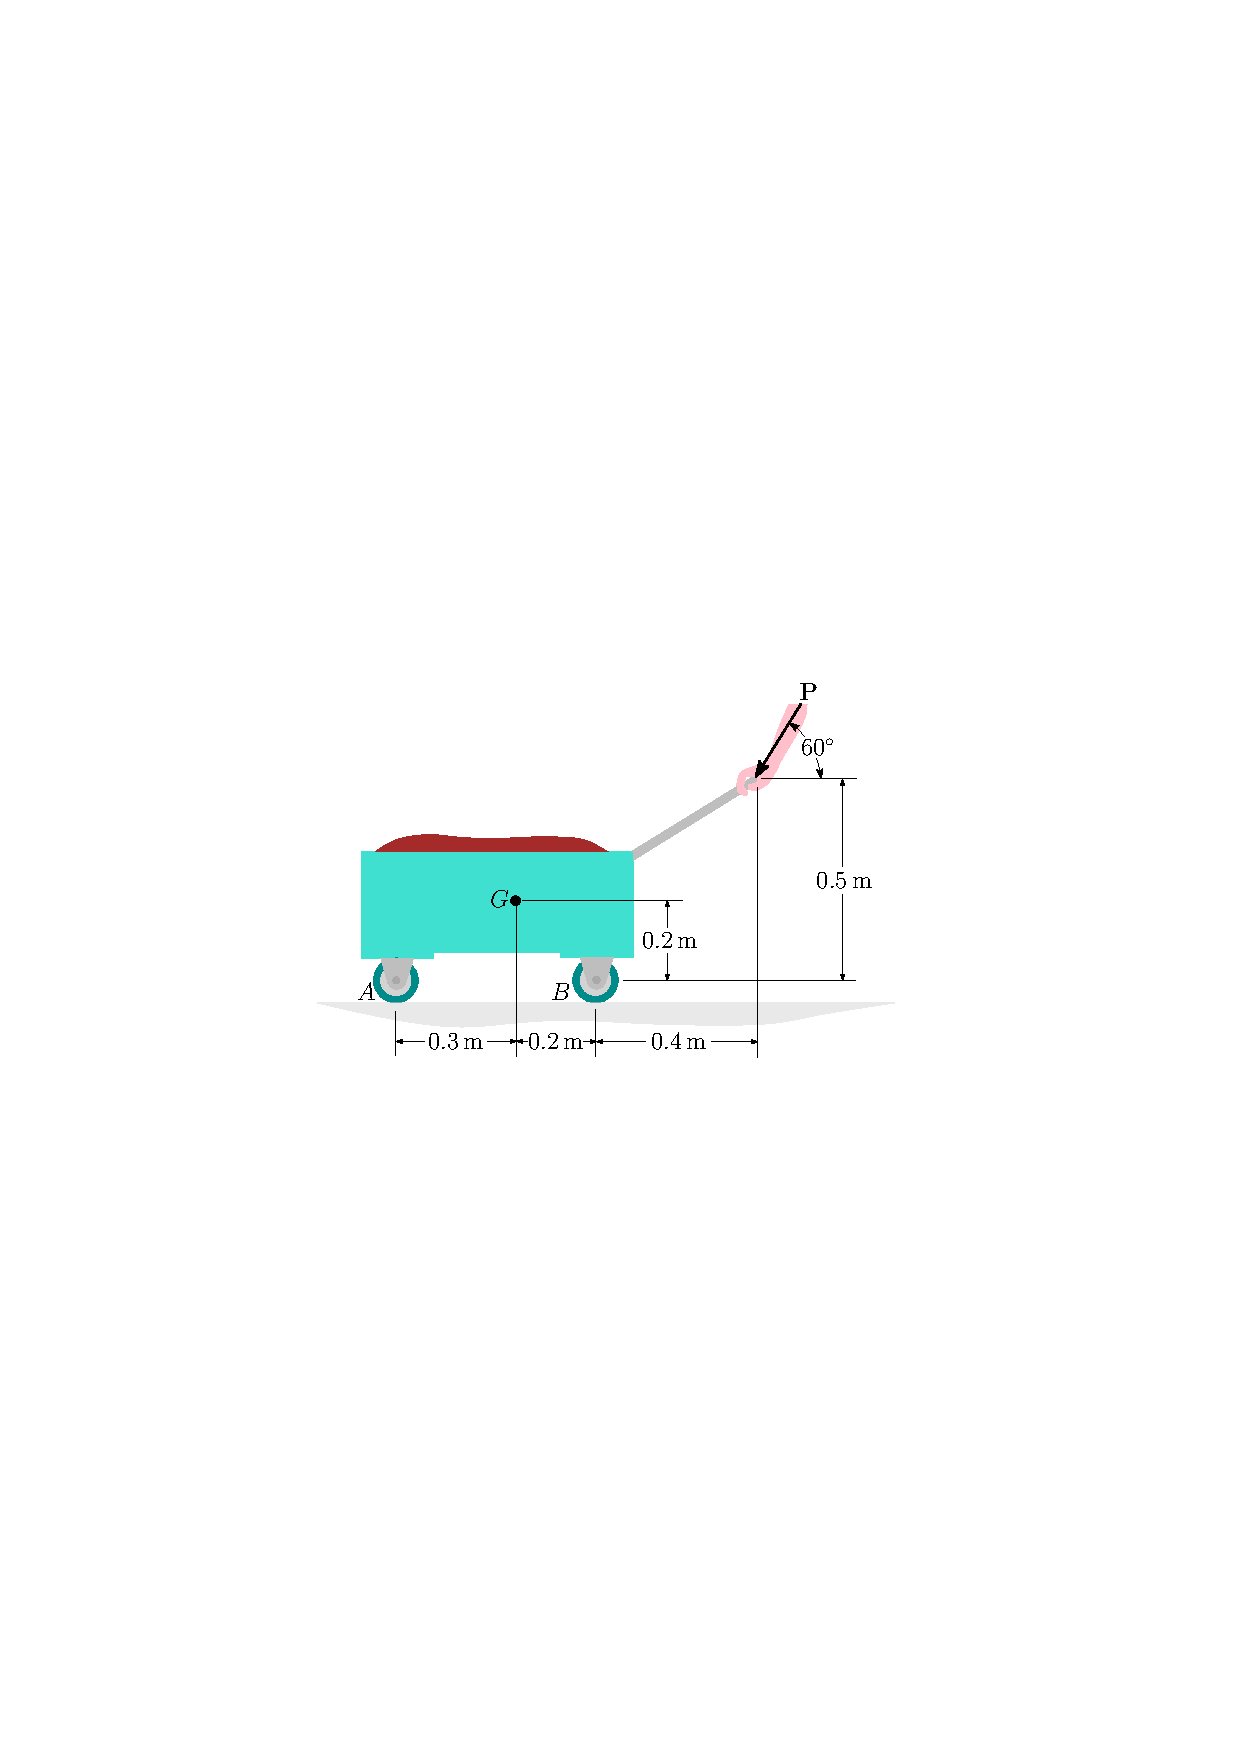
\includegraphics[scale=1.1]{../../images/draw_6}
\end{flushright}
